\subsection{QuizziPedia::Front-End}
\subsubsection{Informazioni generali}
\label{QuizziPedia::Front-End}
\begin{figure}[ht]
	\centering
	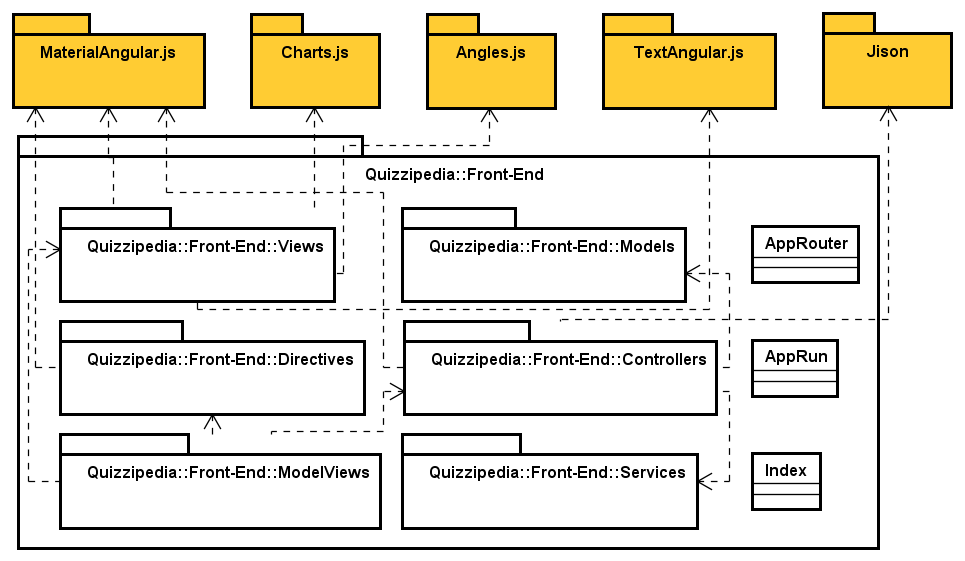
\includegraphics[scale=0.35]{UML/Package/QuizziPedia_Front-end.png}
	\caption{QuizziPedia::Front-End}
\end{figure}
\FloatBarrier
	\begin{itemize}
		\item \textbf{Descrizione}: package\ped{G} contenente le componenti front-end dell'applicazione;
		\item \textbf{Package contenuti}:
		\begin{itemize}
			\item \texttt{Controllers}: package\ped{G} contenente i \textit{controllers\ped{G}} front-end dell'applicazione;
			\item \texttt{Directives}: package\ped{G} contenente le \textit{directives\ped{G}} front-end dell'applicazione;
			\item \texttt{Models}: package\ped{G} contenente le classi che definiscono la business logic dell'applicazione;
			\item \texttt{Services}: package\ped{G} contenente i \textit{services\ped{G}} front-end dell'applicazione;
			\item \texttt{Views}: package\ped{G} contenente le \textit{views\ped{G}} front-end dell'applicazione;
		\end{itemize}
	\end{itemize}

\subsubsection{Classi}
		
	\paragraph{QuizziPedia::Front-End::Index}
	\begin{figure} [ht]
		\centering
		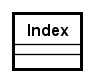
\includegraphics[scale=0.7]{UML/Classi/Front-End/QuizziPedia_Front-end_Views_Index.png}
		\caption{QuizziPedia::Front-End::Views::Index}
	\end{figure} \FloatBarrier
	\begin{itemize}
		\item \textbf{Descrizione}: \textit{view\ped{G}} generale dell'applicazione;
		\item \textbf{Utilizzo}: contiene gli elementi che saranno presenti in ogni pagina dell'applicazione;
		\item \textbf{Relazioni con altre classi}:
		\begin{itemize}
			\item \textbf{IN} \texttt{AppRun}: classe che verifica se l'utente sia autenticato e che abbia le giuste autorizzazioni per la pagina in cui si trova;
			\item \textbf{IN} \texttt{MenuBarDirective}: rappresenta il menù, presente in ogni pagina dell'applicazione, generato in base agli oggetti passati nello \$scope isolato. Fornisce un pulsante per ogni oggetto ricevuto come parametro, ogni pulsante viene rappresentato con un’icona e con un testo. Al click di un pulsante viene invocata la funzione ad esso associata;
			\item \textbf{IN} \texttt{FooterDirective}: \textit{directive\ped{G}} che mostra il footer dell'applicazione che sarà presente in ogni pagina;
			\item \textbf{IN} \texttt{ClickableAreaQuestionsView}: \textit{view\ped{G}} contenente i campi e le direttive per creare una domanda ad area cliccabile;
			\item \textbf{IN} \texttt{ConnectionQuestionsView}: \textit{view\ped{G}} contenente i campi e le direttive per creare una domanda a collegamento;
			\item \textbf{IN} \texttt{CreateQuestionnaireView}: \textit{view\ped{G}} per la creazione del questionario. In questo componente viene permesso anche all'utente di:
			\begin{itemize}
				\item Effettuare delle ricerche sul database di domande;
				\item Selezionare le domande da inserire nel questionario;
				\item Mostrare le domande già inserite e permettere all'utente di eliminarle da tale lista.
			\end{itemize}
			\item \textbf{IN} \texttt{EditorQMLView}: \textit{view\ped{G}} contenente l'editor QML per la creazione di domande personalizzate;
			\item \textbf{IN} \texttt{FillingQuestionnaireView}: \textit{view\ped{G}} principale per la compilazione del questionario; conterrà i vari templates di ogni domanda appartenente al questionario;
			\item \textbf{IN} \texttt{FilligQuestionsView}: \textit{view\ped{G}} contenente i campi e le direttive per creare una domanda a riempimento testo;
			\item \textbf{IN} \texttt{HomeView}: \textit{view\ped{G}} contenente la direttiva per barra di ricerca degli utenti e questionari e il bottone che porterà l'utente nella modalità allenamento;
			\item \textbf{IN} \texttt{ImagesSortingQuestionsView}: \textit{view\ped{G}} contenente i campi e le direttive per creare una domanda a ordinamento immagini;
			\item \textbf{IN} \texttt{LoginView}: \textit{view\ped{G}} contenente le form necessarie per effettuare il login. Contiene inoltre un link alla pagina di registrazione e uno alla pagina per il recupero della password;
			\item \textbf{IN} \texttt{MultipleQuestionsView}: \textit{view\ped{G}} contenente le direttive per creare una domanda a risposta multipla;
			\item \textbf{IN} \texttt{OtherUserView}: \textit{view\ped{G}} contenente le direttive dei dati personali e delle statistiche di un utente ricercato;
			\item \textbf{IN} \texttt{PasswordForgotView}: \textit{view\ped{G}} contenente le form necessarie per il recupero della password dimenticata; 
			\item \textbf{IN} \texttt{ProfileManagementView}: \textit{view\ped{G}} contenente i dati personali che un utente può modificare dopo essersi registrato al sistema;
			\item \textbf{IN} \texttt{QuestionnaireManagementView}:  \textit{view\ped{G}} principale per la gestione dei questionari;
			\item \textbf{IN} \texttt{QuestionsManagementView}: \textit{view\ped{G}} contenente l'elenco delle domande create; 
			\item \textbf{IN} \texttt{RegistrationManagementView}: \textit{view\ped{G}} che permette di visualizzare gli utenti iscritti ad un questionario;
			\item \textbf{IN} \texttt{ResultsQuestionnaireView}: \textit{view\ped{G}} contenente i risultati conseguiti dagli utenti che hanno compilato il proprio questionario;
			\item \textbf{IN} \texttt{ResultsView}: \textit{view\ped{G}} contenente i risultati della ricerca effettuata. Vengono visualizzati sia gli utenti che i questionari trovati;
			\item \textbf{IN} \texttt{SignUp}:  \textit{view\ped{G}} contenente le form dedicate alla registrazione utente. Contiene inoltre un link alla pagina di login;
			\item \textbf{IN} \texttt{StringSortingQuestionsView}:  \textit{view\ped{G}} contenente i campi e le direttive per creare una domanda a ordinamento stringhe; 
			\item \textbf{IN} \texttt{TrainingView}: \textit{view\ped{G}} principale della modalità allenamento; conterrà i vari templates di ogni domanda dell'allenamento;
			\item \textbf{IN} \texttt{TrueFalseQuestionsView}: \textit{view\ped{G}} contenente le direttive per creare una domanda vero/falso;
			\item \textbf{IN} \texttt{UserView}:  \textit{view\ped{G}} contenente le direttive dei dati personali dell'utente, delle sue statistiche relative ai questionari e agli allenamenti effettuati e dei questionari a cui è iscritto.
		\end{itemize}
	\end{itemize}

		\paragraph{QuizziPedia::Front-End::AppRun}
		
		\label{QuizziPedia::Front-End::AppRun}
		
		\begin{figure}[ht]
			\centering
			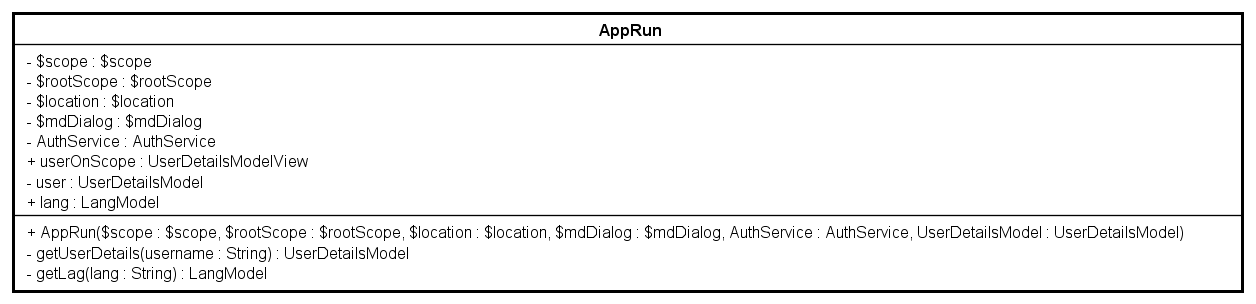
\includegraphics[scale=0.5,keepaspectratio]{UML/Classi/Front-End/QuizziPedia_Front-end_AppRun.png}
			\caption{QuizziPedia::Front-End::AppRun}
		\end{figure} \FloatBarrier
		
		\begin{itemize}
			\item \textbf{Descrizione}: classe che verifica se l'utente sia autenticato e che abbia le giuste autorizzazioni per la pagina in cui si trova;
			\item \textbf{Utilizzo}: viene utilizzata per verificare che l’utente sia autenticato e che abbia la giusta autorizzazione per la pagina in cui si trova;
			\item \textbf{Relazioni con altre classi}: 
			\begin{itemize}
				\item \textbf{IN} \texttt{LangService}: questa classe permette di gestire la lingua nella quale si è scelto di utilizzare l'applicazione;
				\item \textbf{IN} \texttt{LangModel}: rappresenta le informazioni per la giusta traduzione dell'applicazione;
				\item \textbf{IN} \texttt{UserDetailsModel}: rappresenta un utente. Contiene tutte le informazioni necessarie alla presentazione del contenuto di un utente sia nella visualizzazione che nella gestione di un profilo;
				\item \textbf{IN} \texttt{AuthService}: questa classe permette di gestire la registrazione e l'autenticazione di un utente.
			\end{itemize}
			\item \textbf{Attributi}: 
			\begin{itemize}
				\item \texttt{-} \texttt{\$scope: \$scope} \\
				Campo dati contenente un riferimento all'oggetto \$scope creato da \textit{Angular\ped{G}};
				\item \texttt{-} \texttt{\$rootScope: \$rootScope} \\
				Campo dati contenente il riferimento all'oggetto globale \$rootScope creato da \textit{Angular\ped{G}};
				\item \texttt{-} \texttt{\$location: \$location} \\
				Campo dati contenente un riferimento al servizio creato da \textit{Angular\ped{G}} che permette di accedere alla barra degli indirizzi del \textit{browser\ped{G}}, i cambiamenti all'URL nella barra degli indirizzi si riflettono in questo oggetto e viceversa;
				\item \texttt{-} \texttt{\$mdDialog: \$mdDialog} \\
				Campo dati contenente un riferimento al servizio della libreria \textit{Material for Angular\ped{G}} che permette di creare delle componenti a pop-up;
				\item \texttt{-} \texttt{AuthService: AuthService} \\
				Campo dati contenente un riferimento al servizio che si occupa della gestione delle informazioni legate all'autenticazione;
				\item \texttt{+} \texttt{userOnScope: UserDetailsModelView} \\
				Oggetto di tipo \texttt{UserDetailsModelView}. Rappresenta l'oggetto dell'utente autenticato all'interno dello \texttt{\$rootScope};
				\item \texttt{-} \texttt{user: UserDetailsModel} \\
				Oggetto di tipo \texttt{UserDetailsModel}. Rappresenta l'oggetto dell'utente autenticato;
				\item \texttt{+} \texttt{lang: LangModel} \\
				Oggetto di tipo \texttt{LangModel}. Rappresenta l'oggetto contenente la giusta traduzione del template delle pagine.
			\end{itemize}
			\item \textbf{Metodi}: 
			\begin{itemize}
				\item \texttt{+} \texttt{AppRun(\$scope: \$scope, \$rootScope: \$rootScope, \$location: \$location, \$mdDialog: \$mdDialog, AuthService: AuthService, UserDetailsModel: \\UserDetailsModel)} \\
				Metodo costruttore della classe. Recupera dopo il login tutte le informazioni dell'utente. Recupera anche da  \\
				\textbf{Parametri}:
				\begin{itemize}
					\item \texttt{\$scope: \$scope} \\
					Parametro contenente un riferimento all’oggetto \$scope creato da \textit{Angular\ped{G}}. Viene utilizzato come mezzo di comunicazione tra il controller e la view. Contiene gli oggetti che definiscono il viewmodel e il model dell’applicazione;
					\item \texttt{\$rootScope: \$rootScope} \\
					Parametro contenente il riferimento all'oggetto globale \$rootScope creato da \textit{Angular\ped{G}};
					\item \texttt{\$location: \$location} \\
					Parametro contenente un riferimento al servizio creato da \textit{Angular\ped{G}} che permette di accedere alla barra degli indirizzi del \textit{browser\ped{G}}, i cambiamenti all’URL nella barra degli indirizzi si riflettono in questo oggetto e viceversa;
					\item \texttt{\$mdDialog: \$mdDialog} \\
					Parametro contenente un riferimento al servizio della libreria \textit{Material for Angular\ped{G}} che permette di creare delle componenti a pop-up;
					\item \texttt{AuthService: AuthService} \\
					Parametro contenente un riferimento al servizio che si occupa della gestione delle informazioni legate all’autenticazione;
					\item \texttt{UserDetailsModel: UserDetailsModel} \\
					Parametro contenente un riferimento alla classe per poter istanziare un oggetto di tipo \texttt{UserDetailsModel}.
				\end{itemize}
				\item \texttt{-} \texttt{getUserDetails(username: String): UserDetailsModel} \\ Metodo che permette di ottenere i dati con una chiamata a \texttt{UserDetailsService};
				\textbf{Parametri}:
				\begin{itemize}
					\item \texttt{username: String}: parametro che identifica l'utente del quale saranno scaricati i dati.
				\end{itemize}
				\item \texttt{-} \texttt{getLag(lang: String): LangModel} \\ Metodo che permette di ottenere i dati con una chiamata a \texttt{LangService}; \\
				\textbf{Parametri}:
				\begin{itemize}
					\item \texttt{lang: String}: parametro che identifica la lingua del sistema.
				\end{itemize}
			\end{itemize}
		\end{itemize}
		
	
	\paragraph{QuizziPedia::Front-End::AppRouter}
	
	\label{QuizziPedia::Front-End::AppRouter}
	
	\begin{figure}[ht]
		\centering
		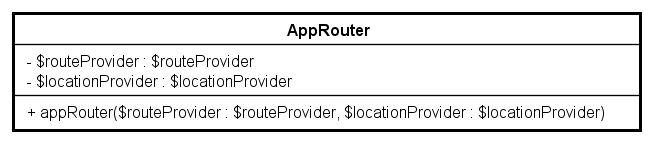
\includegraphics[scale=0.5,keepaspectratio]{UML/Classi/Front-End/QuizziPedia_Front-end_AppRouter.png}
		\caption{QuizziPedia::Front-End::AppRouter}
	\end{figure} \FloatBarrier
	
	\begin{itemize}
		\item \textbf{Descrizione}: classe che gestisce i routes dell’applicazione, utilizza il servizio \$routeProvider per associare ad ogni route un controller e una view;
		\item \textbf{Utilizzo}: viene utilizzata per associare un URL alle varie view dell’applicazione;
		\item \textbf{Metodi}: 
		\begin{itemize}
			\item \texttt{-} \texttt{appRouter(\$routeProvider: \$routeProvider, \$locationProvider: \$locationProvider)}: metodo che gestisce i routes dell’applicazione. Utilizza il servizio \$routeProvider per associare ad ogni route un controller e una view; e \$locationProvider per configurare come i paths dell'applicazione vengono salvati. Questa funzione viene utilizzata come parametro nel metodo texttt{config} di \textit{Angular.js}. Il metoto \texttt{config} permette di impostare l'esecuzione di una funzione al caricamento del \textit{modulo\ped{G}} principale di \textit{Angular.js\ped{G}};
			\textbf{Metodi}:
			\begin{itemize}
				\item \texttt{\$routeProvider}: campo dati contenente un riferimento al servizio di \textit{Angular.js\ped{G}} che si occupa di definire le route dell’applicazione;
				\item \texttt{\$locationProvider}: campo dati contenente un riferimento al servizio di \textit{Angular.js\ped{G}} che si occupa di configuare come i paths vengono memorizzati;
			\end{itemize}
		\end{itemize}
	\end{itemize}
	
